%%% LaTeX Template: Article/Thesis/etc. with colored headings and special fonts
%%%
%%% Source: http://www.howtotex.com/
%%%
%%% Modified January 2016 by CDM
%%% Restructured 2026 by CDM to follow ISO/IEC/IEEE 42010:2022 (Architecture description)
%%% and IEEE Std 1016-2009 (Software Design Descriptions)

%%%  Preamble
\documentclass[11pt,letterpaper]{article}
\usepackage[margin=1.0in]{geometry}
\usepackage[T1]{fontenc}
\usepackage[bitstream-charter]{mathdesign}
\usepackage[latin1]{inputenc}
\usepackage{amsmath}
\usepackage{xcolor}
\usepackage{cite}
\usepackage{hyphenat}
\usepackage{graphicx}
\usepackage{float}
\usepackage{subfigure}
\usepackage{sectsty}
\usepackage[compact]{titlesec}
\usepackage[tablegrid]{vhistory}
\usepackage{pbox}
\usepackage{longtable}
\allsectionsfont{\color{accentcolor}\scshape\selectfont}

%%% Definitions
\definecolor{accentcolor}{rgb}{0.0,0.0,0.5}
\newcommand{\teamname}{Team Name}
\newcommand{\productname}{Product Name}
\newcommand{\coursename}{CSE 4316: Senior Design I}
\newcommand{\semester}{Fall 2026}
\newcommand{\docname}{Architectural Design Specification}
\newcommand{\department}{Department of Computer Science \& Engineering}
\newcommand{\university}{The University of Texas at Arlington}
\newcommand{\authors}{Alan Turing \\ Grace Hopper \\ John Von Neumann \\ Ada Lovelace \\ Charles Babbage}

%%% Headers and footers
\usepackage{fancyhdr}
	\pagestyle{fancy}						% Enabling the custom headers/footers
\usepackage{lastpage}
	% Header (empty)
	\lhead{}
	\chead{}
	\rhead{}
	% Footer
	\lfoot{\footnotesize \teamname \ - \semester}
	\cfoot{}
	\rfoot{\footnotesize page \thepage\ of \pageref{LastPage}}	% "Page 1 of 2"
	\renewcommand{\headrulewidth}{0.0pt}
	\renewcommand{\footrulewidth}{0.4pt}

%%% Change the abstract environment
\usepackage[runin]{abstract}			% runin option for a run-in title
\abslabeldelim{\quad}
\setlength{\abstitleskip}{-10pt}
\renewcommand{\abstractname}{}
\renewcommand{\abstracttextfont}{\color{accentcolor} \small \slshape}	% slanted text

%%% Start of the document
\begin{document}

%%% Cover sheet
{\centering \huge \color{accentcolor} \sc \textbf{\department \\ \university} \par}
\vspace{1 in}
{\centering \huge \color{accentcolor} \sc \textbf{\docname \\ \coursename \\ \semester} \par}
\vspace{0.5 in}
\begin{figure}[h!]
	\centering
   	
\includegraphics[width=0.60\textwidth]{images/test_image}
\end{figure}
\vspace{0.5 in}
{\centering \huge \color{accentcolor} \sc \textbf{\teamname \\ \productname} \par}
\vspace{0.5 in}
{\centering \large \sc \textbf{\authors} \par}
\newpage

%%% Revision History
\begin{versionhistory}
  	\vhEntry{0.1}{10.01.2026}{GH}{document creation}
  	\vhEntry{0.2}{10.05.2026}{AT|GH}{complete draft}
  	\vhEntry{0.3}{10.12.2026}{AT|GH}{release candidate 1}
  	\vhEntry{1.0}{10.20.2026}{AT|GH|CB}{official release}
  	\vhEntry{1.1}{10.31.2026}{AL}{added design review requests}
\end{versionhistory}
\newpage

%%% Table of contents
\setcounter{tocdepth}{2}
\tableofcontents
\newpage

%%% List of figures and tables (optional)
\listoffigures
\listoftables
\newpage

%%% NOTE TO STUDENTS (remove before submission):
%%% This template follows the architecture description conventions of
%%% ISO/IEC/IEEE 42010:2022 (stakeholders, concerns, architecture viewpoints,
%%% architecture views, decisions and rationale) and the design viewpoints of
%%% IEEE Std 1016-2009. The system is described as a set of architecture VIEWS,
%%% each governed by a VIEWPOINT that frames specific stakeholder CONCERNS. The
%%% familiar X/Y/Z layer decomposition is presented as the logical/functional
%%% view of the architecture.

%%% Document sections
\section{Introduction}
This Architectural Design Specification (ADS) describes the software and system architecture of \productname. It is organized as an \textit{architecture description} in the sense of ISO/IEC/IEEE 42010:2022 \cite{ISO42010} and draws its design viewpoints from IEEE Std 1016-2009 \cite{IEEE1016}. The architecture is presented as a set of complementary \textit{views}, each governed by a \textit{viewpoint} that frames the concerns of specific stakeholders.

Your introduction should describe the product concept in sufficient detail that the architectural design is easy to follow. The introduction may reuse the product overview from the System Requirements Specification (SRS) for this purpose. At a minimum, state the product concept, scope, and key requirements, and reference the SRS and Project Charter so the reader can locate the driving requirements. Avoid detailed implementation choices (specific components, languages) here --- those belong to the Detailed Design Specification.

\subsection{Purpose \& Scope}
State the purpose of this document and the scope of the architecture it describes. Identify what is inside the architecture's boundary and what is treated as an external actor or system.

\subsection{Applicable Documents}
Reference the SRS (source of requirements), the Project Charter (source of constraints and objectives), and any external standards or interface control documents the architecture must conform to.

\newpage
\section{Stakeholders \& Architectural Concerns}
ISO/IEC/IEEE 42010:2022 \cite{ISO42010} requires that an architecture description identify the system's \textit{stakeholders} and the \textit{concerns} they hold about the architecture. Concerns are the interests --- such as functionality, performance, safety, security, cost, maintainability, or regulatory compliance --- that the architecture must address. Each concern is later framed by one or more architecture viewpoints (Section 3) and answered by the corresponding views (Sections 4--8).

\subsection{Stakeholders}
Identify each stakeholder or stakeholder role that has an interest in the architecture. Typical roles include the customer/sponsor, end users, the development team, maintainers, the course instructor, and any external system owners.

\subsection{Architectural Concerns}
List the concerns held by the stakeholders above. Focus on concerns that shape architectural decisions (not detailed requirements). The matrix below maps stakeholders to their concerns; use it to confirm every significant concern has an owner and is addressed by at least one view.

\begin{table}[H]
\caption{Stakeholder / concern matrix}
\begin{center}
    \begin{tabular}{ | p{4cm} | p{9cm} |}
    \hline
    \textbf{Stakeholder} & \textbf{Primary concerns} \\ \hline
    Customer / sponsor & functionality delivered, cost, schedule, fitness for purpose \\ \hline
    End users & usability, responsiveness, reliability \\ \hline
    Development team & feasibility, modularity, testability \\ \hline
    Maintainers & modifiability, observability, documentation \\ \hline
    (add roles) & (add concerns) \\ \hline
    \end{tabular}
\end{center}
\end{table}

\newpage
\section{Architecture Viewpoints}
An \textit{architecture viewpoint} (ISO/IEC/IEEE 42010:2022 \cite{ISO42010}) establishes the conventions for constructing and interpreting one kind of \textit{view}: which stakeholders and concerns it frames, and the model kinds (notations) it uses. This section declares the viewpoints used in the remainder of the document. Each subsequent section is a view that conforms to one of these viewpoints. The viewpoints below combine the 42010 framework with the design viewpoints of IEEE Std 1016-2009 \cite{IEEE1016}; adapt the set to your project.

\begin{table}[H]
\caption{Architecture viewpoints used in this document}
\begin{center}
    \begin{tabular}{ | p{3cm} | p{5cm} | p{2.5cm} | p{2.5cm} |}
    \hline
    \textbf{Viewpoint} & \textbf{Frames (concerns)} & \textbf{Model kind} & \textbf{Realized in} \\ \hline
    Context & system boundary, external actors/systems & context diagram & Section 4 \\ \hline
    Composition / Data Flow & decomposition into layers/subsystems and the data exchanged & block \& data-flow diagram & Section 5 \\ \hline
    Logical / Functional & responsibilities and interfaces of each subsystem & block diagram, interface tables & Sections 6--8 \\ \hline
    Deployment & mapping of software to hardware/nodes & deployment diagram & Section 7 or 8 (as needed) \\ \hline
    \end{tabular}
\end{center}
\end{table}

\subsection{Architectural Style \& Conventions}
Describe the overall architectural strategy for the system: the top-level decomposition into \textit{layers}. An architectural layer is the top-level logical view, or abstraction, of the design. Layers are composed of related elements of similar capability, are highly independent of other layers, and have clearly defined interfaces and interactions. Each layer is identified individually and is unique in its function and purpose within the system.

State the naming conventions your team will use for layers, subsystems, modules, interfaces, and data flows, and the interface identifier scheme (e.g. \texttt{\#01}, \texttt{\#02}) referenced by the subsystem interface tables in Sections 6--8. Consistent conventions here make the views, the Detailed Design Specification, and the traceability matrix easy to cross-reference.

\newpage
\section{System Overview \& Context View}
This section presents the \textbf{context view} and the top-level structure of the system. The context view (conforming to the Context viewpoint declared in Section 3) fixes the system boundary and shows the external actors and systems that interact with \productname. The layer descriptions then give the overall structure of the software system --- the strategy for how it will be built.

\begin{figure}[h!]
	\centering
 	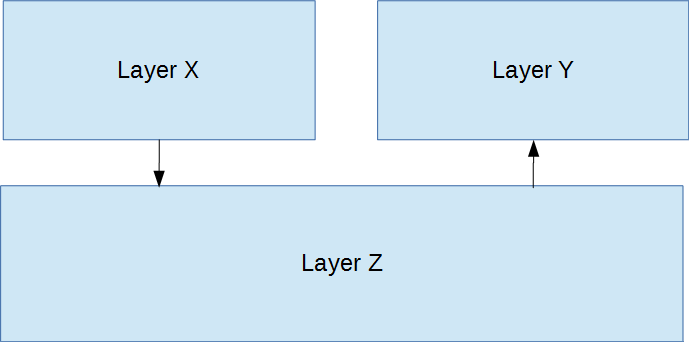
\includegraphics[width=0.60\textwidth]{images/layers}
 \caption{Architectural layer diagram}
\end{figure}

An architectural ``layer'' is the top-level logical view, or abstraction, of your design. Layers should be composed of related elements of similar capability, should be highly independent of other layers, and should have clearly defined interfaces and interactions with other layers. Each layer is identified individually and is unique in its function and purpose within the system. Provide the high-level block diagram of the layers above, and describe the function of each layer below.

\subsection{Layer X Description}
Describe this layer in detail: its features, functions, and the services it provides, and its critical interfaces and interactions with adjacent layers. Note any architecturally significant properties (e.g. this layer is the only one permitted to touch external hardware, or persistent storage).

\subsection{Layer Y Description}
Describe this layer in detail, following the same pattern as Layer X.

\subsection{Layer Z Description}
Describe this layer in detail, following the same pattern as Layer X. Ensure the set of layers is complete (every major responsibility belongs to exactly one layer) and that inter-layer interfaces are consistent with the data-flow view in Section 5.

\newpage
\section{Subsystem Definitions \& Data Flow}
This section breaks down your layer abstraction to another level of detail. Here you grapically represent the logical subsytems that compose each layer and show the interactions/interfaces between those subsystems. A subsystem can be thought of as a programming unit that implements one of the major functions of the layer. It, therefore, has data elements that serve as source/sinks for other subsystems. The logical data elements that flow between subsystems need to be explicitly defined at this point, beginning with a data flow-like diagram based on the block diagram.

\begin{figure}[h!]
	\centering
 	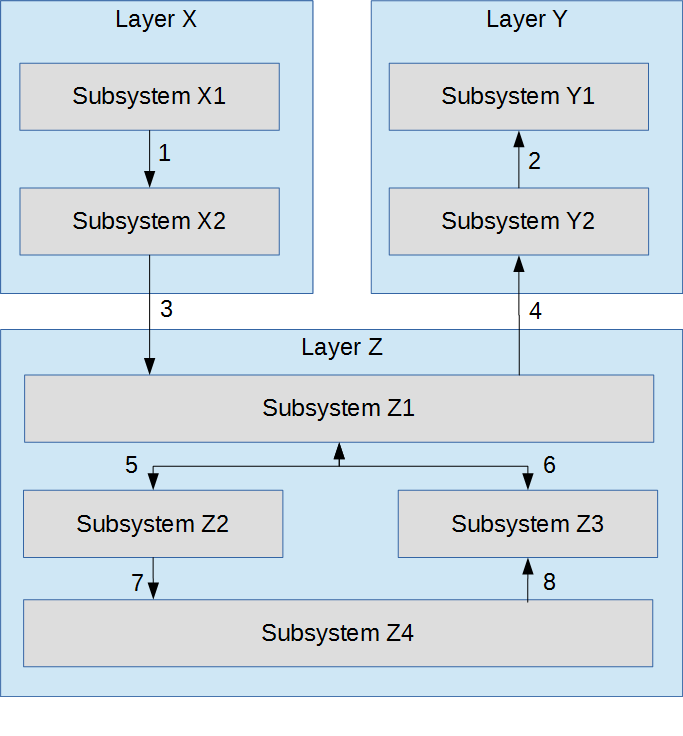
\includegraphics[width=\textwidth]{images/data_flow}
 \caption{A simple data flow diagram}
\end{figure}

\newpage
\section{X Layer Subsystems}
This section is the \textbf{logical/functional view} of the X layer (conforming to the Logical/Functional viewpoint declared in Section 3). The layer is decomposed into its subsystems, and the responsibilities, interfaces, and data flows of each subsystem are defined. A subsystem is a programming unit that implements one of the major functions of the layer and serves as a source/sink of data for other subsystems. Describe each subsystem in a separate subsection using the same structure. Include any special considerations or trade-offs for the approach chosen.

\subsection{Subsystem 1}
A general description of this subsystem. For most subsystems, an extract of the architectural block diagram with data flows is useful --- showing this subsystem and those it communicates with.

\begin{figure}[h!]
	\centering
 	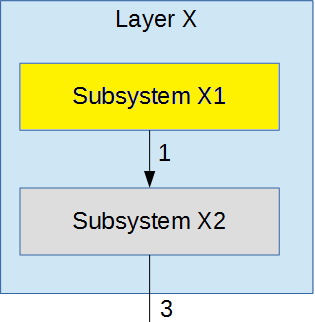
\includegraphics[width=0.60\textwidth]{images/subsystem}
 \caption{Example subsystem description diagram}
\end{figure}

\subsubsection{Assumptions}
Any assumptions made in defining the subsystem. Pay particular attention to assumptions concerning interfaces and interactions with other layers.

\subsubsection{Responsibilities}
Expand each responsibility/feature/function/service of this subsystem, as identified in the architectural overview, into more detailed responsibilities. Clearly describe what the subsystem does (and does not do).

\subsubsection{Subsystem Interfaces}
Define each input and output for the subsystem. Create one row per labelled interface that connects to this subsystem, describing the incoming and outgoing data elements. Interface identifiers use the scheme declared in Section 3 and are the anchors for requirements traceability.

\begin {table}[H]
\caption {Subsystem interfaces}
\begin{center}
    \begin{tabular}{ | p{1cm} | p{6cm} | p{3cm} | p{3cm} |}
    \hline
    ID & Description & Inputs & Outputs \\ \hline
    \#01 & Description of the interface/bus & \pbox{3cm}{input 1 \\ input 2} & \pbox{3cm}{output 1}  \\ \hline
    \#02 & Description of the interface/bus & \pbox{3cm}{N/A} & \pbox{3cm}{output 1}  \\ \hline
    \end{tabular}
\end{center}
\end{table}

\subsubsection{Design Rationale}
Briefly justify this subsystem's boundary and approach: why these responsibilities are grouped together, and any significant alternatives considered. Record architecturally significant choices as decisions in Section 9 and reference them here (e.g. ``per AD-02'').

\subsection{Subsystem 2}
Repeat for each subsystem.

\subsection{Subsystem 3}
Repeat for each subsystem.

\newpage
\section{Y Layer Subsystems}
This section is the \textbf{logical/functional view} of the Y layer (conforming to the Logical/Functional viewpoint declared in Section 3). The layer is decomposed into its subsystems, and the responsibilities, interfaces, and data flows of each subsystem are defined. A subsystem is a programming unit that implements one of the major functions of the layer and serves as a source/sink of data for other subsystems. Describe each subsystem in a separate subsection using the same structure. Include any special considerations or trade-offs for the approach chosen.

\subsection{Subsystem 1}
A general description of this subsystem. For most subsystems, an extract of the architectural block diagram with data flows is useful --- showing this subsystem and those it communicates with.

\begin{figure}[h!]
	\centering
 	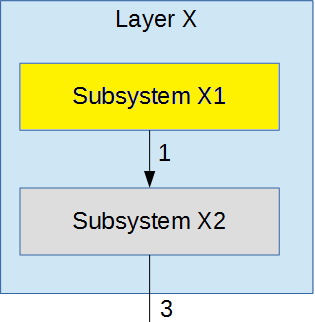
\includegraphics[width=0.60\textwidth]{images/subsystem}
 \caption{Example subsystem description diagram}
\end{figure}

\subsubsection{Assumptions}
Any assumptions made in defining the subsystem. Pay particular attention to assumptions concerning interfaces and interactions with other layers.

\subsubsection{Responsibilities}
Expand each responsibility/feature/function/service of this subsystem, as identified in the architectural overview, into more detailed responsibilities. Clearly describe what the subsystem does (and does not do).

\subsubsection{Subsystem Interfaces}
Define each input and output for the subsystem. Create one row per labelled interface that connects to this subsystem, describing the incoming and outgoing data elements. Interface identifiers use the scheme declared in Section 3 and are the anchors for requirements traceability.

\begin {table}[H]
\caption {Subsystem interfaces}
\begin{center}
    \begin{tabular}{ | p{1cm} | p{6cm} | p{3cm} | p{3cm} |}
    \hline
    ID & Description & Inputs & Outputs \\ \hline
    \#01 & Description of the interface/bus & \pbox{3cm}{input 1 \\ input 2} & \pbox{3cm}{output 1}  \\ \hline
    \#02 & Description of the interface/bus & \pbox{3cm}{N/A} & \pbox{3cm}{output 1}  \\ \hline
    \end{tabular}
\end{center}
\end{table}

\subsubsection{Design Rationale}
Briefly justify this subsystem's boundary and approach: why these responsibilities are grouped together, and any significant alternatives considered. Record architecturally significant choices as decisions in Section 9 and reference them here (e.g. ``per AD-02'').

\subsection{Subsystem 2}
Repeat for each subsystem.

\subsection{Subsystem 3}
Repeat for each subsystem.

\newpage
\section{Z Layer Subsystems}
This section is the \textbf{logical/functional view} of the Z layer (conforming to the Logical/Functional viewpoint declared in Section 3). The layer is decomposed into its subsystems, and the responsibilities, interfaces, and data flows of each subsystem are defined. A subsystem is a programming unit that implements one of the major functions of the layer and serves as a source/sink of data for other subsystems. Describe each subsystem in a separate subsection using the same structure. Include any special considerations or trade-offs for the approach chosen.

\subsection{Subsystem 1}
A general description of this subsystem. For most subsystems, an extract of the architectural block diagram with data flows is useful --- showing this subsystem and those it communicates with.

\begin{figure}[h!]
	\centering
 	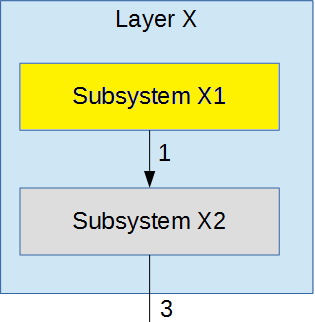
\includegraphics[width=0.60\textwidth]{images/subsystem}
 \caption{Example subsystem description diagram}
\end{figure}

\subsubsection{Assumptions}
Any assumptions made in defining the subsystem. Pay particular attention to assumptions concerning interfaces and interactions with other layers.

\subsubsection{Responsibilities}
Expand each responsibility/feature/function/service of this subsystem, as identified in the architectural overview, into more detailed responsibilities. Clearly describe what the subsystem does (and does not do).

\subsubsection{Subsystem Interfaces}
Define each input and output for the subsystem. Create one row per labelled interface that connects to this subsystem, describing the incoming and outgoing data elements. Interface identifiers use the scheme declared in Section 3 and are the anchors for requirements traceability.

\begin {table}[H]
\caption {Subsystem interfaces}
\begin{center}
    \begin{tabular}{ | p{1cm} | p{6cm} | p{3cm} | p{3cm} |}
    \hline
    ID & Description & Inputs & Outputs \\ \hline
    \#01 & Description of the interface/bus & \pbox{3cm}{input 1 \\ input 2} & \pbox{3cm}{output 1}  \\ \hline
    \#02 & Description of the interface/bus & \pbox{3cm}{N/A} & \pbox{3cm}{output 1}  \\ \hline
    \end{tabular}
\end{center}
\end{table}

\subsubsection{Design Rationale}
Briefly justify this subsystem's boundary and approach: why these responsibilities are grouped together, and any significant alternatives considered. Record architecturally significant choices as decisions in Section 9 and reference them here (e.g. ``per AD-02'').

\subsection{Subsystem 2}
Repeat for each subsystem.

\subsection{Subsystem 3}
Repeat for each subsystem.

\newpage
\section{Architecture Decisions \& Rationale}
ISO/IEC/IEEE 42010:2022 \cite{ISO42010} calls for an architecture description to record the \textit{architecture decisions} and their \textit{rationale} --- the reasoning, alternatives considered, and trade-offs behind the architecture. Capturing decisions here makes the architecture reviewable and gives future maintainers the ``why'' behind the structure. Record each architecturally significant decision using the lightweight format below (an architecture decision record).

\subsection{AD-01: [Decision Title]}
\begin{itemize}
  \item \textbf{Context:} The situation and forces (requirements, constraints, concerns) that made a decision necessary.
  \item \textbf{Decision:} The choice that was made, stated plainly.
  \item \textbf{Alternatives considered:} Other options evaluated and why they were not chosen.
  \item \textbf{Consequences:} The resulting trade-offs --- positive and negative --- and any concerns (from Section 2) that remain only partially addressed.
  \item \textbf{Affected concerns / requirements:} Stakeholder concerns and SRS requirement IDs influenced by this decision.
\end{itemize}

\subsection{AD-02: [Decision Title]}
Repeat for each architecturally significant decision (for example: choice of layering, monolith vs. service decomposition, synchronous vs. message-based communication, on-device vs. cloud processing, primary datastore, safety-interlock strategy).

\newpage
\section{Requirements Traceability}
This section provides forward traceability from the requirements baseline (SRS) to the architectural elements that realize each requirement. It confirms that every significant requirement is addressed by at least one subsystem, and that every subsystem exists to satisfy identified requirements. Maintain this matrix as the architecture evolves; the Detailed Design Specification extends it down to individual components, and the Test Plan links requirements to test cases.

\begin{table}[H]
\caption{Requirement-to-architecture traceability (excerpt)}
\begin{center}
    \begin{tabular}{ | p{2cm} | p{5.5cm} | p{5cm} |}
    \hline
    \textbf{Req ID} & \textbf{Requirement (abbreviated)} & \textbf{Realizing subsystem(s)} \\ \hline
    FR-01 & abbreviated requirement text & X Layer / Subsystem 1 \\ \hline
    PE-01 & abbreviated requirement text & Y Layer / Subsystem 2 \\ \hline
    SE-01 & abbreviated requirement text & Z Layer / Subsystem 1 \\ \hline
    \end{tabular}
\end{center}
\end{table}

\newpage

%%% References
\bibliographystyle{reference/IEEEtran_custom}
\bibliography{reference/refs}{}

\end{document}
